%%%%%%%%%%%%%%%%%%%%%%%%%%%%%%%%%%%%%%
%%%%%%%%%%%%%%%%%%%%%%%%%%%%%%%%%%%%%%
% Do not edit the TeX file your work
% will be overwritten.  Edit the RnW
% file instead.
%%%%%%%%%%%%%%%%%%%%%%%%%%%%%%%%%%%%%%
%%%%%%%%%%%%%%%%%%%%%%%%%%%%%%%%%%%%%%
  


We demonstrate the local sensitivity computations on a 
Gaussian mixture model (GMM) of the iris data set. 
The data set is a sample of 150 iris flowers with 
four measurements taken per flower:  
sepal length, sepal width, petal length, and petal width. 
The generative model and variational approximation for the GMM 
were detailed in 
\exref{iris_bnp_process,iris_var_distr}, respectively, 
with data dimension $d = 4$ and truncation parameter $\kmax = 15$. 
\figref{iris_fit} shows the GMM fit at $\alpha = 6$. 
The data set contains three iris species, and
the BNP model correspondingly identifies three dominant clusters. 


\begin{knitrout}
\definecolor{shadecolor}{rgb}{0.969, 0.969, 0.969}\color{fgcolor}\begin{figure}[!h]

{\centering 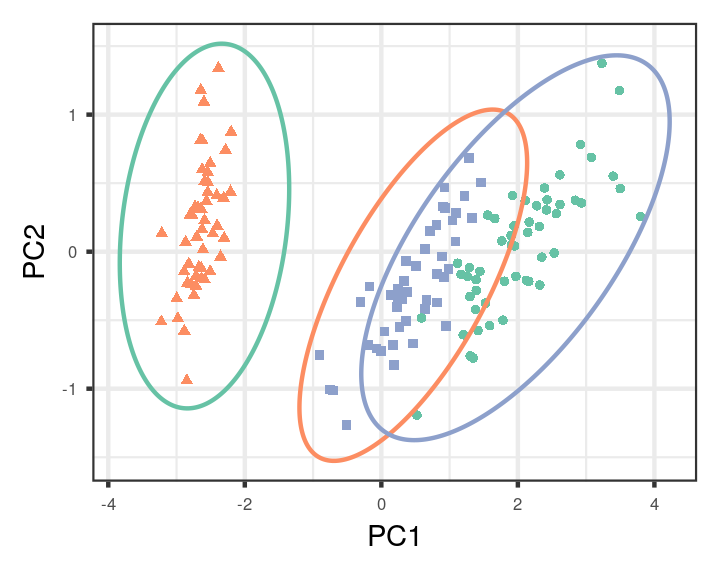
\includegraphics[width=0.588\linewidth,height=0.470\linewidth]{figure/iris_fit-1} 

}

\caption[The iris data in principal component space and 
                      GMM fit at $\alpha = 6$]{The iris data in principal component space and 
                      GMM fit at $\alpha = 6$. 
                      Colors denote inferred memberships and
                      ellipses represent estimated covariances. }\label{fig:iris_fit}
\end{figure}


\end{knitrout}


We wish to evaluate the sensitivity of the expected number of clusters to the 
stick-breaking distribution. 
Define the expected number of \textit{in-sample} clusters as
\begin{align*}
\gclusters(\eta)
&= \expect{\q(\z\vert\eta)}{\sum_{k=1}^\kmax \ind{ \left(\sum_{n=1}^{N}
\z_{\n\k}\right) > 0}} \\ 
&= \sum_{k=1}^\kmax \left(1 -  \prod_{n=1}^N
\left(1 - \expect{\q(\z_{nk}\vert\eta)}{\z_{nk}}\right)\right).
\end{align*}

The in-sample quantity $\gclusters$ is an estimate for 
the number of species present in the observed iris data set. 
Alternatively, we can define a {\itshape posterior predictive} quantity, 
which is an estimate of the number of species one would expect to see 
should a new iris data set of size $N$ be collected.
Define the posterior predictive number of clusters as 
\begin{align}\eqlabel{post_pred_nclusters}
\gclusterspred(\eta) = \expect{\q(\nu\vert\eta)}{\sum_{k=1}^\kmax\left(1 -
(1 - \pi_k)^N\right)},
\end{align}
where recall that $\pi_k$ are the mixture weights computed from the stick-lengths, $\pi_\k = \nuk \prod_{\k' < \k} (1 - \nu_{\k'})$. 

Unlike the in-sample quantity, the expectation for the predictive quantity is not a simple closed-form function of the variational parameters.  
Instead, we approximated \eqref{post_pred_nclusters} using Monte Carlo draws from the variational distribution. 
Specifically, we used the ``reparameterization trick"
to sample from the variational distribution:
we constructed an $\eta$-dependent transformation 
$f(\cdot, \eta)$ that satisfies 
\begin{align*}
  u \iid\normdist{0, I} \implies 
  f(u, \eta) \stackrel{d}{=} \nu \sim \q(\cdot | \eta).
\end{align*}
Since $\nu$ is a vector of logit-normal random variables under $q$, 
we let $f(\cdot ; \eta)$ be a function that scales and shifts the normal draws $u$ according to parameters in $\eta$;
it then applies the sigmoid function to the 
scaled and shifted draws. 

To form a Monte Carlo estimate of \eqref{post_pred_nclusters}, 
we sampled $u_1, \dots, u_m\stackrel{iid}{\sim}\normdist{0, I}$ 
and then averaged the expression inside the expectation evaluated at points 
$f(u_1, \eta), \ldots, f(u_m, \eta)$.
We used the reparameterization trick so that conditional on $u_1, \ldots, u_m$,
our Monte Carlo estimate of $\gclusterspred$ is a determinstic function of 
the variational parameters $\eta$. 
In our experiments below, all displayed values of $\gclusterspred(\eta)$ are
Monte Carlo approximations, 
conditional on the same $m = 10,000$ draws $u_1, \ldots, u_m$, fixed a priori. 

We first evaluate the sensitivity of the posterior quantities 
$\gclusters$ and $\gclusterspred$ to the prior parameter $\alpha$. 
We fit the initial variational posterior at $\alpha_0 = 6$,
and we formed the linear approximation (\eqref{vb_eta_sens}) at this initial fit. 
Without further optimization, we use the linear approximation to quickly evaluate 
$\etalin(\alpha)$ for all $\alpha = 1, \ldots, 16$ (\eqref{etalin_def}),
and produce posterior quantites $g(\etalin(\alpha))$. 

The in-sample quantity appears insensitive to changes in the $\alpha$ parameter
(\figref{iris_alpha_sens}). 
As $\alpha$ varies from $\alpha = 1, \ldots, 16$,
the quantity $\gclusters(\etalin(\alpha))$
varies only from 3.0 to
3.4
(recall that the true number of iris species is three). 
On the other hand, the posterior preditive quantity is sensitive 
to changes in $\alpha$.
Over the same range of $\alpha$, $\gclusterspred(\etalin(\alpha))$
varies from 
3.6 to 
8.1. 


Subsequent refits at $\alpha\not=\alpha_0$ confirm sensitivity conclusions of the linear approximation. 
Over the range $\alpha = 1, \ldots, 16$,
the values $g(\etalin(\alpha))$ closely mimic the 
values $g(\etaopt(\alpha))$ found by refitting 
the variational parameters at each $\alpha$ (\figref{iris_alpha_sens}).
Importantly, 
the linear approximation is an order of magnitude faster than refitting. 
Forming the linear approximation at $\alpha = \alpha_0$, 
required 0.02 seconds. 
After forming the linear approximation,
computing $\etalin(\alpha)$ for all $\alpha = 1, \ldots, 16$ took another 
0.02 seconds.
On the other hand, to refit $\etaopt(\alpha)$ for the same range of
$\alpha$'s took a total of  9 seconds, with a median refit time of 0.6 seconds. 









\begin{knitrout}
\definecolor{shadecolor}{rgb}{0.969, 0.969, 0.969}\color{fgcolor}\begin{figure}[!h]

{\centering 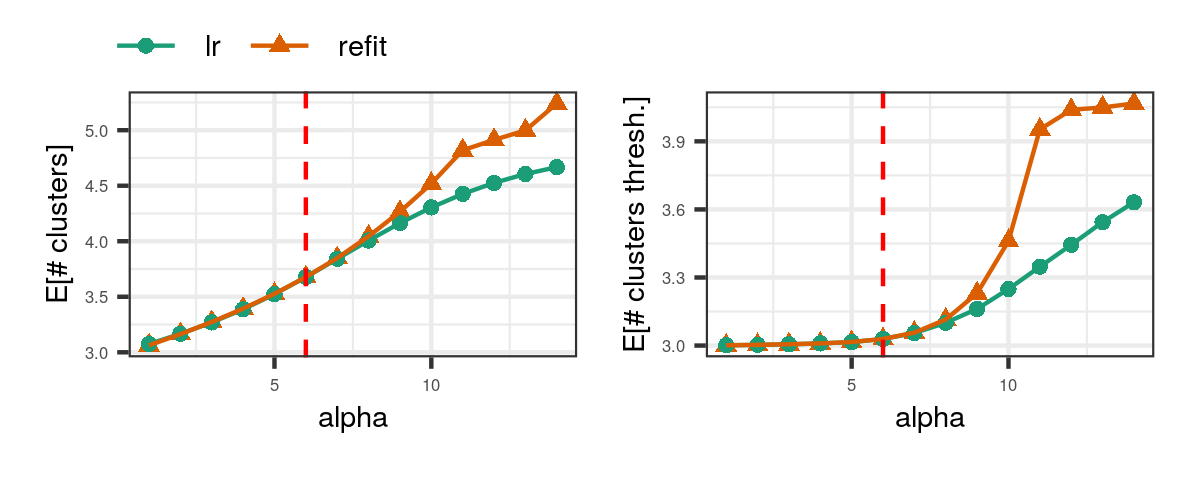
\includegraphics[width=0.784\linewidth,height=0.439\linewidth]{figure/iris_alpha_sens-1} 

}

\caption[The expected number of clusters as $\alpha$ varies in the 
the GMM fit of the iris data]{The expected number of clusters as $\alpha$ varies in the 
the GMM fit of the iris data. 
On the left is in-sample quantity $\gclusters$.  
On the right is the the predictive quantity $\gclusterspred$. 
We formed the linear approximation at $\alpha=6$. 
In red, the expected number of clusters computed under the
linearly approximated variational parameters (red).
In blue, the expected number of clusters obtained by refitting the model at each $\alpha$. }\label{fig:iris_alpha_sens}
\end{figure}


\end{knitrout}


% 
% - we demonstrate the utility of the influence function 
% - figure ref top three rows shows three different functional perturbations. 
% - can't really tell from densities how these will affect posterior statistic
% - but they do in fact have very different effects (in sign and size). 
% - but their effects make sense when looking at the influence function
% 
% -last row is worst-case

We next examine functional perturbations,
and we demonstrate the ability of the influence function to 
provide guidance on the anticipated effect of potential perturbations 
on a posterior quantity. 
We consider functional perturbations of the form 
$\phi_\mu(x) = e^{2(x - \mu)^2}$, with each perturbation having a 
different mode $\mu$ (\figref{iris_fsens} left column). 
The perturbations are multiplicative with perturbed prior 
$p(\nu_k|\t) = p_0(\nu_k)\exp(\t\phi_\mu(\nu_k))$.
The middle column of \figref{iris_fsens} displays the initial density,
$p_0(\nu_k) = \betadist{\nu_k\vert 1, \alpha_0}$,
along with the perturbed densities
$p(\nu_k|\t = 1)$ for different choices of $\mu$. 

Each perturbation $\phi_\mu$ with a different choice of $\mu$ 
produces distinct changes in the expected number
of in-sample clusters $\gclusters$. 
The right column of \figref{iris_fsens} plots the differences
$\gclusters(\etaopt(\t)) - \gclusters(\etaopt(0))$ 
for $\t\in[0,1]$, where $\etaopt(\t)$ are variational parameters
fitted under the perturbed stick-distribution $p(\nu_k|\t)$.
Depending on the perturbation, 
the change in $\gclusters$ can be positive, negative, or nearly zero. 
In each case, the approximation 
$\gclusters(\etalin(\t)) - \gclusters(\etalin(0))$
is able to mirror the qualitative behavior observed under refitting.

\todo{depending on what has been said about influence functions before, we may need a more thorough discussion below}

While each perturbation produces distinct changes in $\gclusters$, 
it is difficult to anticipate the effect of the perturbation 
by comparing the original and perturbed densities alone. 
However, the sign and magnitude of the change in $\gclusters$ after 
prior perturbation are well-explained by its influence function
(\figref{iris_fsens} left column). 
When $\phi_\mu$ is centered at a location where the influence function is negative, the effect of the perturbation on $\gclusters$ 
is negative (\figref{iris_fsens} top row); 
conversely, when $\phi_\mu$ is centered at a location where the influence function is positive, its effect on $\gclusters$ is positive (bottom row); 
finally, when $\phi_\mu$ is centered at a location where the influence transitions from negative to positive, its effect on
$\gclusters$ is roughly zero (middle row). 
In the last case, $\phi_\mu$ placed approximately equal weight on the negative and positive portions of the prior-weighted influence function, resulting in an approximately zero inner-product (\eqref{TODO}). 
In the other data applications below, 
the influence function will guide our choice of functional perturbaton and explain why some perturbations result in greater sensitivity than others. 

Finally, we consider the 
worst-case multiplicative perturbation with unit $L_\infty$ norm.
Recall that the worst-case perturbation with unit $L_\infty$ norm is a 
step-function taking on values $\pm1$ corresponding 
to the sign of the influence function (\figref{iris_worstcase} left).  
The middle column of \figref{iris_worstcase} shows the prior density perturbed by the worst-case perturbation; 
the right column shows the effect on $\gclusters$. 
This worst-case perturbation has a much larger effect on
$\gclusters$ compared to the other unit $L_\infty$ norm perturbations in
\figref{iris_fsens}. 
However, even with the worst-case perturbation, 
the change in $\gclusters$ is still small.
We conclude that on the iris data set, $\gclusters$ appears to be a quantity insensitive to the prior under a Gaussian mixture model. 



\begin{knitrout}
\definecolor{shadecolor}{rgb}{0.969, 0.969, 0.969}\color{fgcolor}\begin{figure}[!h]

{\centering 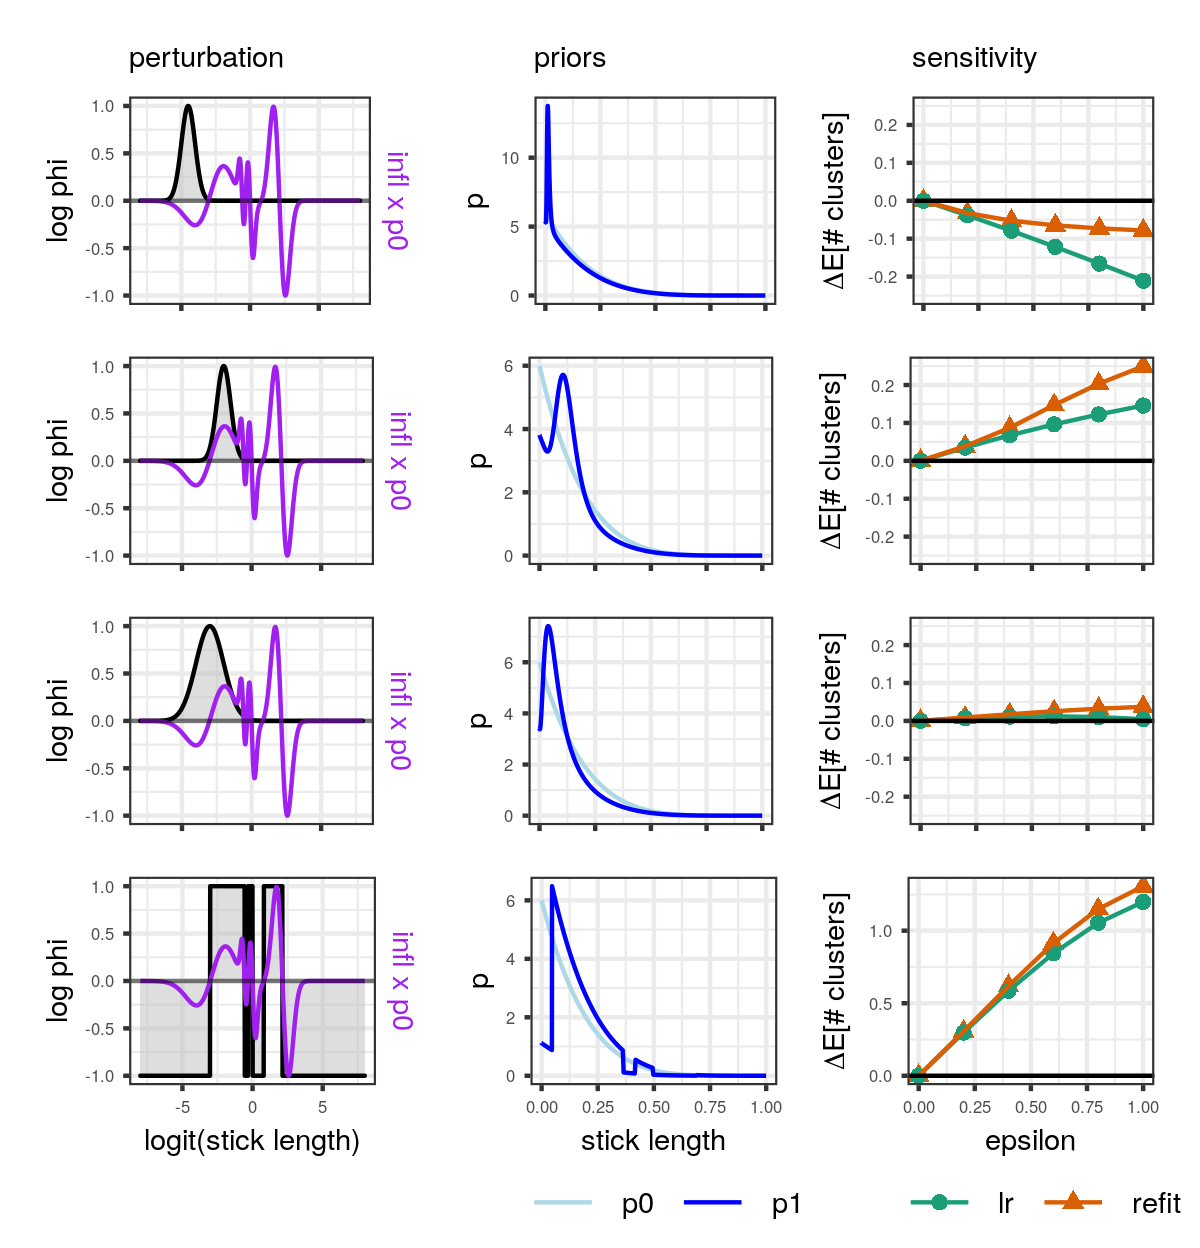
\includegraphics[width=0.980\linewidth,height=0.862\linewidth]{figure/iris_fsens-1} 

}

\caption{Sensitivity of
        the expected number of in-sample clusters 
        in the iris data set
        to three multiplicative perturbations with 
        unit $L_{\infty}$-norm.
        (Left) the multiplicative perturbation $\phi$ in grey.        
        The influence function $\Psi$ in purple, 
        scaled to also have unit $L_{\infty}$-norm. 
        (Middle) the original prior density $\p_0$ and 
        the perturbed prior density $\p_t = \p_0\times \exp(t \phi)$
        at $t = 1$. 
        (Right) the effect of the perturbation 
        on the change in expected number of in-sample clusters 
        as $t\rightarrow1$.}\label{fig:iris_fsens}
\end{figure}


\end{knitrout}


\begin{knitrout}
\definecolor{shadecolor}{rgb}{0.969, 0.969, 0.969}\color{fgcolor}\begin{figure}[!h]

{\centering 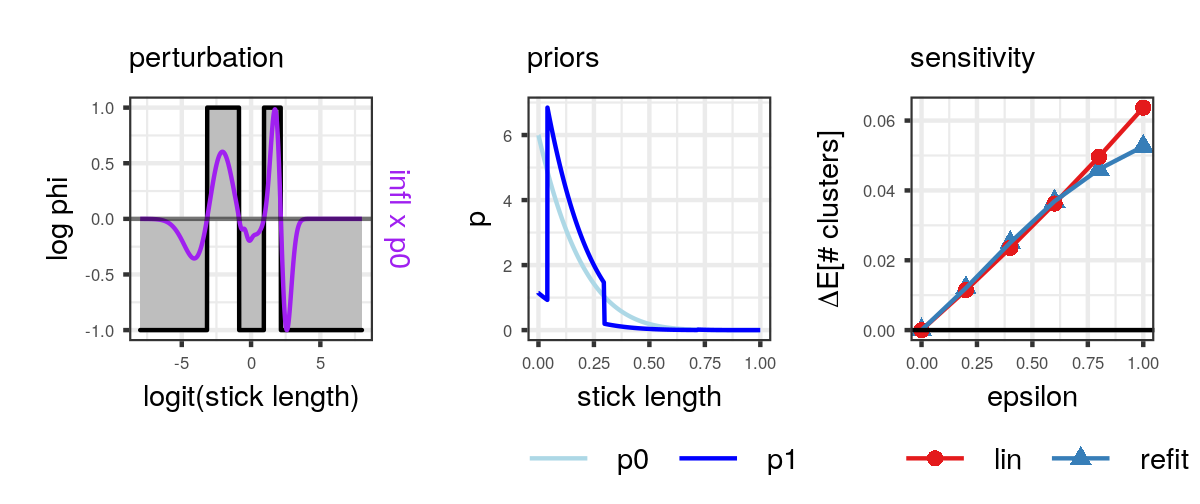
\includegraphics[width=0.980\linewidth,height=0.412\linewidth]{figure/iris_worstcase-1} 

}

\caption[Sensitivity of
        the expected number of in-sample clusters in the iris data set
        to the worst-case multiplicative perturbation with 
        unit $L_{\infty}$-norm]{Sensitivity of
        the expected number of in-sample clusters in the iris data set
        to the worst-case multiplicative perturbation with 
        unit $L_{\infty}$-norm.}\label{fig:iris_worstcase}
\end{figure}


\end{knitrout}

% \begin{table}[tb]
% \centering
% \caption{Compute time of results on the iris data set. }
% \begin{tabular}{|r|r|}
%     \hline 
%     & time (seconds) \\ 
%     \hline 
%     Initial fit & sprintf('%1.2g', init_fit_time) \\
%     \hline 
%     Hessian solve for $\alpha$ sensitivity & 
%         sprintf('%1.2g', alpha_hess_time)\\
%     Linear approx. $\eta^{lin}(\alpha)$ for $\alpha = 1, \ldots , 16$ & 
%         sprintf('%1.2g', total_alpha_lr_time)\\
%     Refits $\eta(\alpha)$ for $\alpha = 1, \ldots , 16$ & 
%         sprintf('%1.2g', total_alpha_refit_time)\\
%     \hline 
%     The influence function & sprintf('%1.2g', infl_time)\\ 
%     Hessian solve for worst-case $\phi$ & 
%         sprintf('%1.2g', wc_hessian_time)\\
%     Linear approx. $\eta^{lin}(\t)|_{\t = 1}$
%     for worst-case $\phi$ & 
%         sprintf('%1.2g', wc_lr_time)\\
%     Refit $\eta(\t)|_{\t = 1}$ for worst-case $\phi$ & 
%         sprintf('%1.2g', wc_refit_time)\\ 
%     \hline 
% \end{tabular}
% \end{table}

